\ylDisplay{Tasapinnaline plaat} % Ülesande nimi
{EFO žürii} % Autor
{piirkonnavoor} % Voor
{2018} % Aasta
{P 4} % Ülesande nr.
{3} % Raskustase
{
% Teema: Valgusõpetus
\ifStatement
Tasapinnaline plaat lõigati kaheks tükiks nagu on näidatud joonisel. Tekkisid kumerlääts ja nõguslääts. Pärast seda nihutati läätsed teineteisest eemale. Mis juhtub paralleelsete kiirte kimbuga, kui see langeb läätsede süsteemile: \\
a) koondava läätse poolt; \\
b) hajutava läätse poolt. \\
Kirjeldage juhte, kui läätsede vahemaa on fookuskaugusest suurem ja väiksem (Kokku neli juhtu).
\ifSolution
\begin{center}
	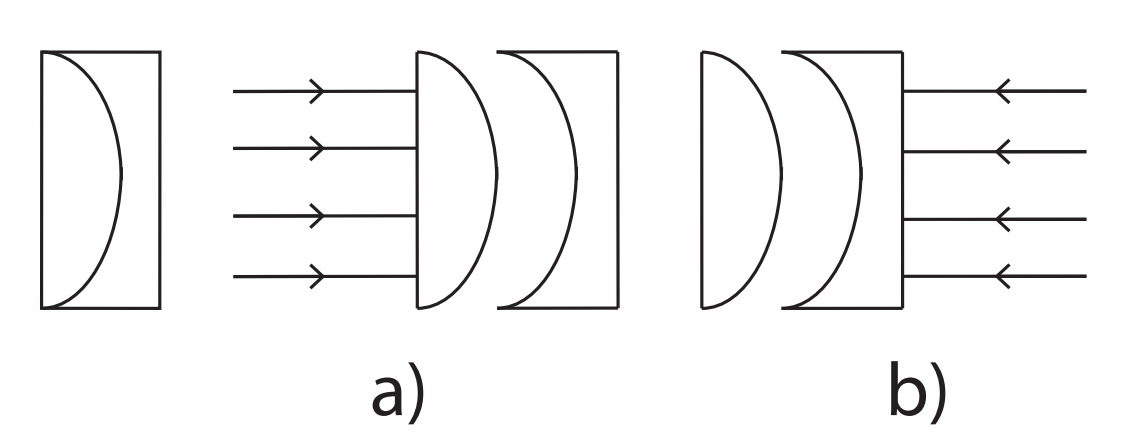
\includegraphics[width=0.5\linewidth]{2018-v2p-04-yl.PNG}
\end{center}
\fi
\ifHint
Tasaparalleelsele plaadile langev valgus väljub plaadist ikka paralleelsena. Kui me vaatleme nüüd plaati koosnevana kumer- ja nõgusläätsest, mis on teineteisest eemale nihutamata, siis näeme, et kumerlääts koondab valgusvihu. Nõgusläätsel on näiv fookus ja kui nõgusläätse fookus langeb kokku kumerläätse fookusega, siis pärast nõgusläätse on valguskiired paralleelsed. Seega lõigatud kumer- ja nõgusläätsel on sama fookuskaugus.
\fi
\ifSolution
Tasaparalleelsele plaadile langev valgus väljub plaadist ikka paralleelsena. Kui me vaatleme nüüd plaati koosnevana kumer- ja nõgusläätsest, mis on teineteisest eemale nihutamata, siis näeme, et kumerlääts koondab valgusvihu. Nõgusläätsel on näiv fookus ja kui nõgusläätse fookus langeb kokku kumerläätse fookusega, siis pärast nõgusläätse on valguskiired paralleelsed. Seega lõigatud kumer- ja nõgusläätsel on sama fookuskaugus. Juht 
a). Kiired langevad kumerläätse poolt. Nihutame läätsed teineteisest veidi eemale. Kumerläätse fookus nihkub lähemale nõgusläätsele, nõgusläätsele langevad koonduvad kiired, mis pärast murdumist on ikka koonduvad, kuigi kiirte koondumispunk on nüüd läätsest kaugemal võrreldes ainult kumerläätsega. Viime läätsed teineteisest veelgi rohkem eemale. Kumerläätsele langenud paralleelsed kiired koonduvad kahe läätse vahelises ruumis ja hajutavale läätsele langevad hajuvad kiired. Pärast nõgusläätse on kiirte hajumine läätsele langenud kiirte hajumisest suurem. 
Juht 
b) Kiired langevad nõgusläätse poolt. Pärast nõgusläätse hajuvad sellele langenud paralleelsed kiired nii, et nende pikendused koonduvad läätse ees fookuses. Kui selles punktis asub ka kumerläätse fookus, siis pärast kumerläätse on valguskiired paralleelsed. Kui läätsed eemaldada teineteisest, siis fookused enam ei kattu ja kumerläätsele langevad hajuvad kiired, mis koonduvad kuskil läätse taga. Kiired koonduvad sõltumata sellest, kui kaugel läätsed teineteisest on.
\fi
}
